% Chapter 4

\chapter{RESULTADOS} % Main chapter title

\label{Chapter4} % For referencing the chapter elsewhere, use \ref{Chapter1} 

%----------------------------------------------------------------------------------------
\section{Importancia del AGN}

\begin{figure}[H]
\centering
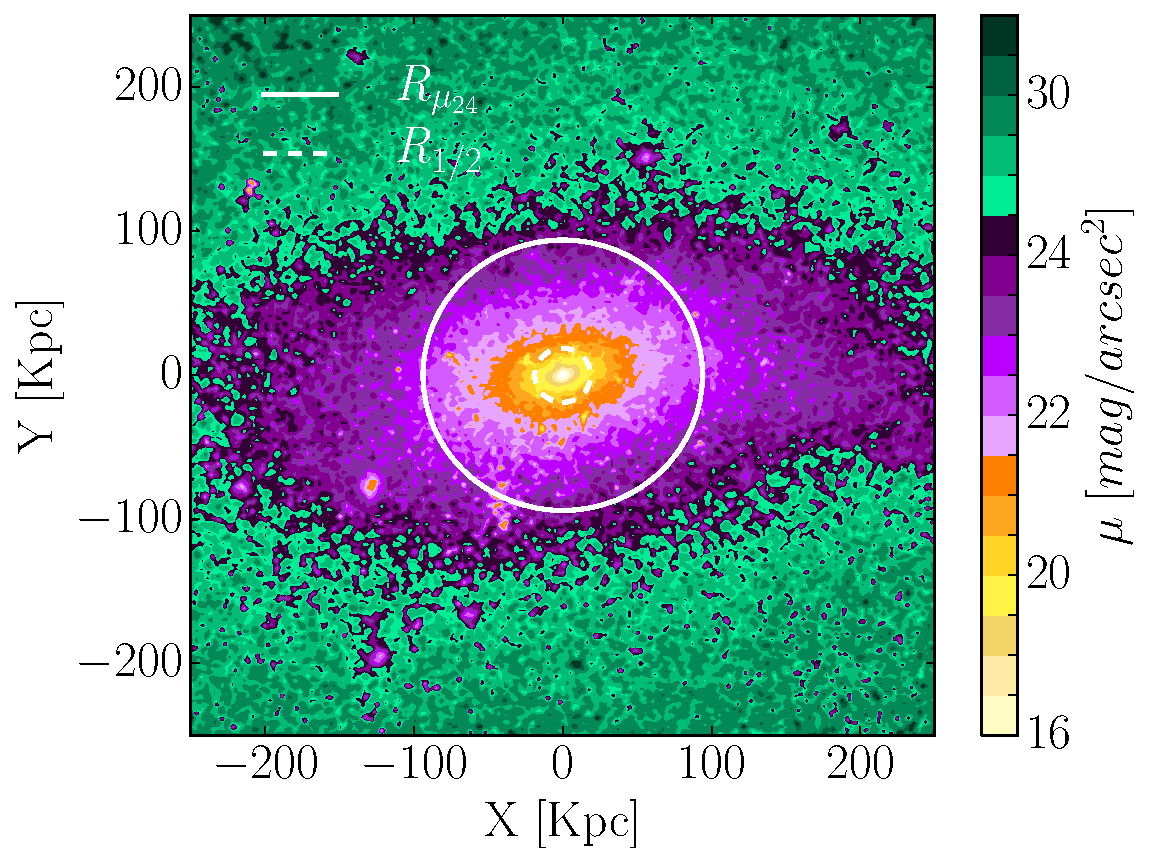
\includegraphics[height=7cm,width=8.5cm,trim={0cm 2cm 3.3cm 0cm},clip]{Figures/d1csf.pdf}
%\hspace*{-0.9cm}
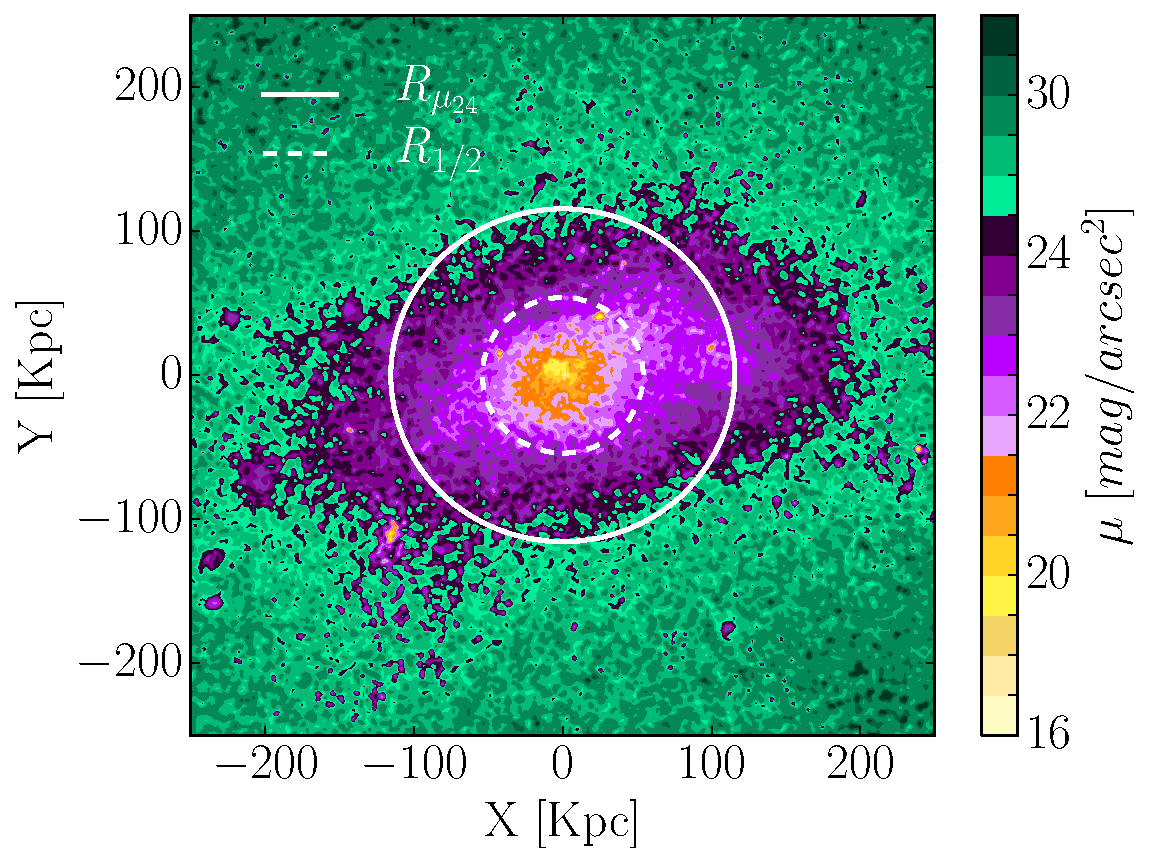
\includegraphics[height=7cm,width=8.5cm,trim={3.1cm 2cm 0cm 0cm},clip]{Figures/d1agn.pdf}
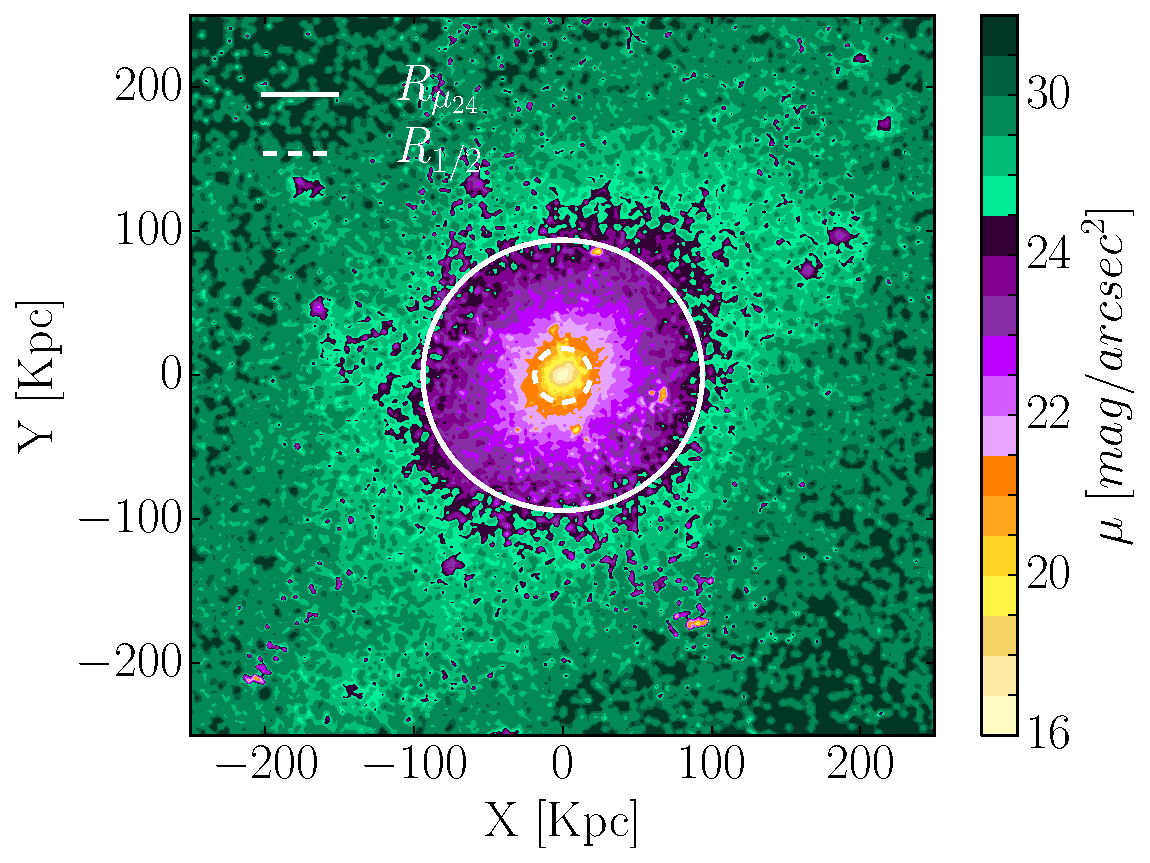
\includegraphics[height=8cm,width=8.5cm,trim={0cm 0cm 3.3cm 0cm},clip]{Figures/d2csf.pdf}
%\hspace*{-0.9cm}
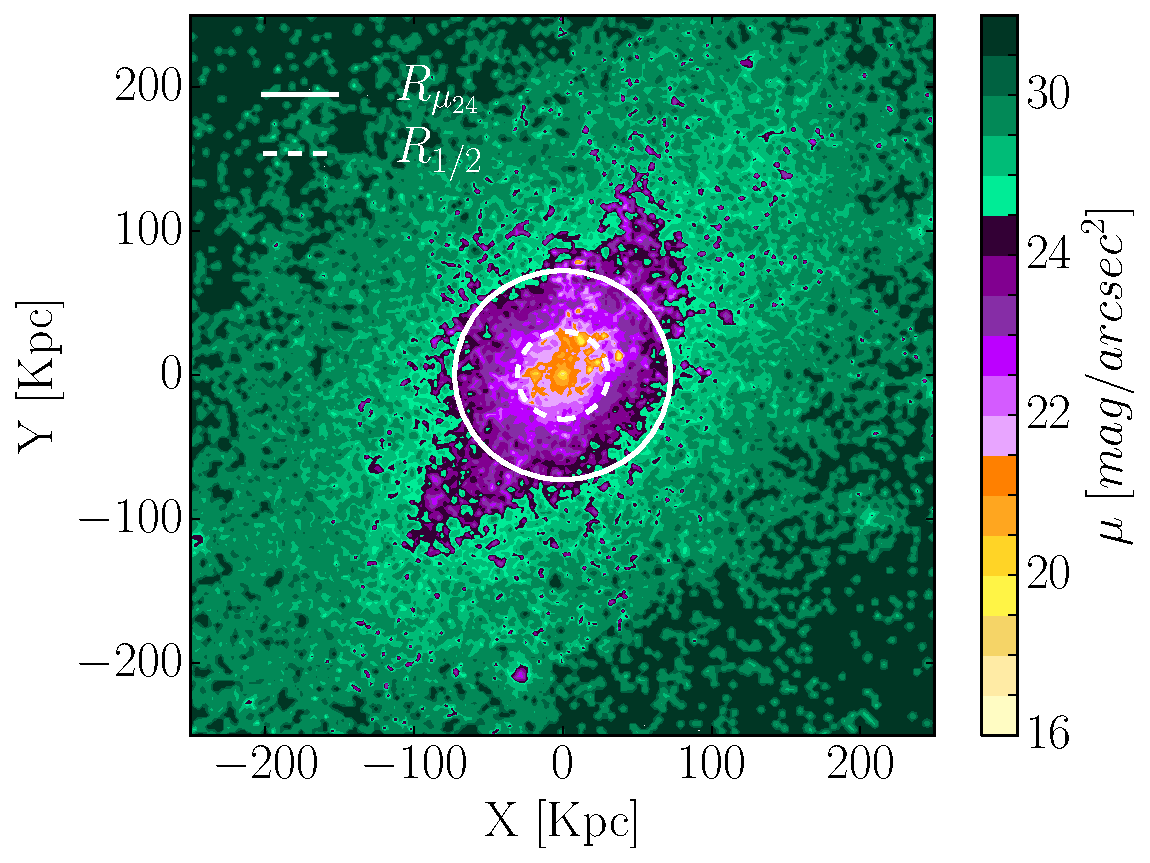
\includegraphics[height=8cm,width=8.5cm,trim={3.1cm 0cm 0cm 0cm},clip]{Figures/d2agn.pdf}
\caption[csfagn]{Lknlnjkl}
\label{fig:csfagn}
\end{figure}

\begin{figure}[H]
\centering
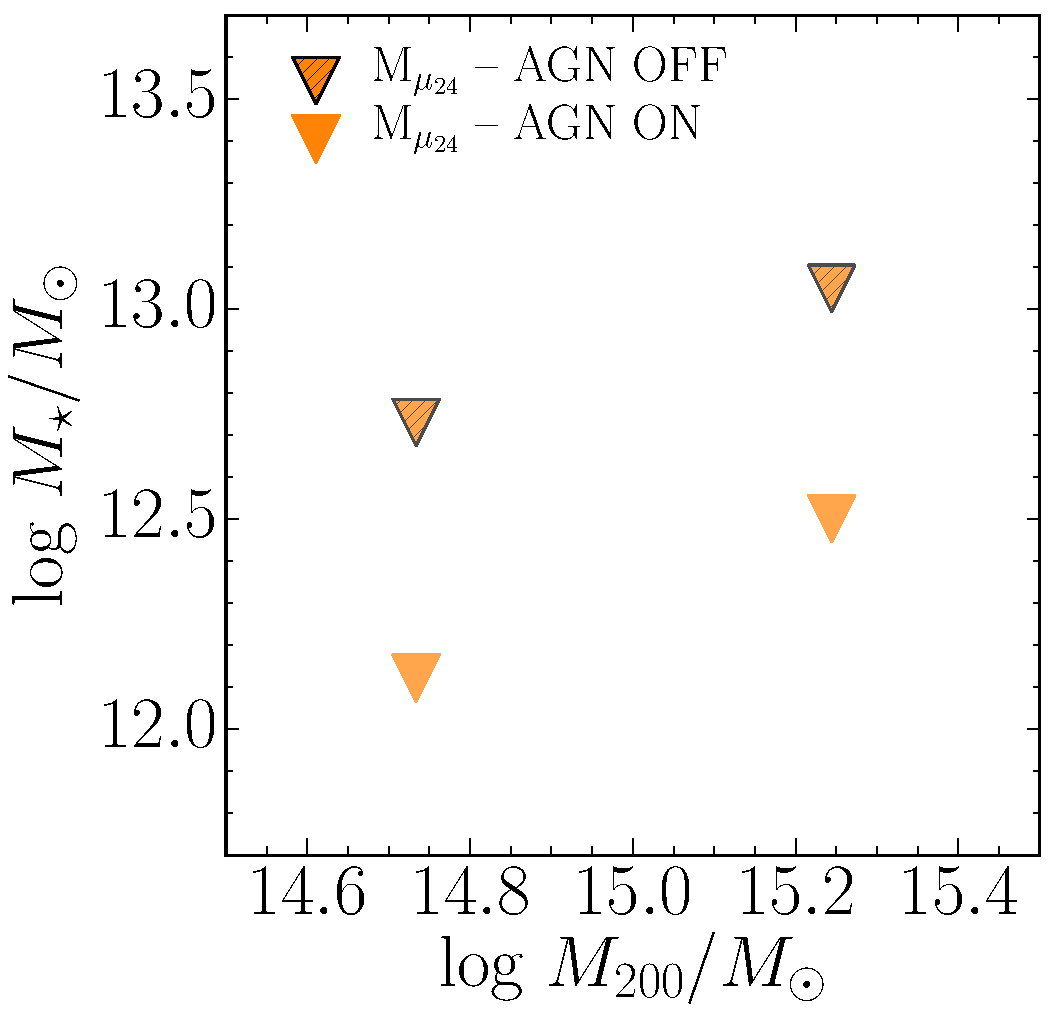
\includegraphics[height=12cm,width=12cm]{Figures/LR/csf_agn.pdf}
%\decoRule
\caption[agn]{La presenta figura muestra la variaci\'on en masa estelar de las BCGs correspondientes a dos regiones,
una grande y una chica. Se puede apreciar c\'omo el hecho de coonsiderar procesos de reatroalimentaci\'on
por {\it AGN} (tria\'angulos anaranjados sin rayas) implica sistem\'aticamente la disminuci\'on de la masa
estelar respecto a considerar s\'olo procesos de reatoalimentaci\'on por supernovas (tri\'angulos anaranjados con rayas)}
\label{fig:agn}
\end{figure}


%----------------------------------------------------------------------------------------

\section{Evoluci\'on Masas}

\begin{figure}[H]
\centering
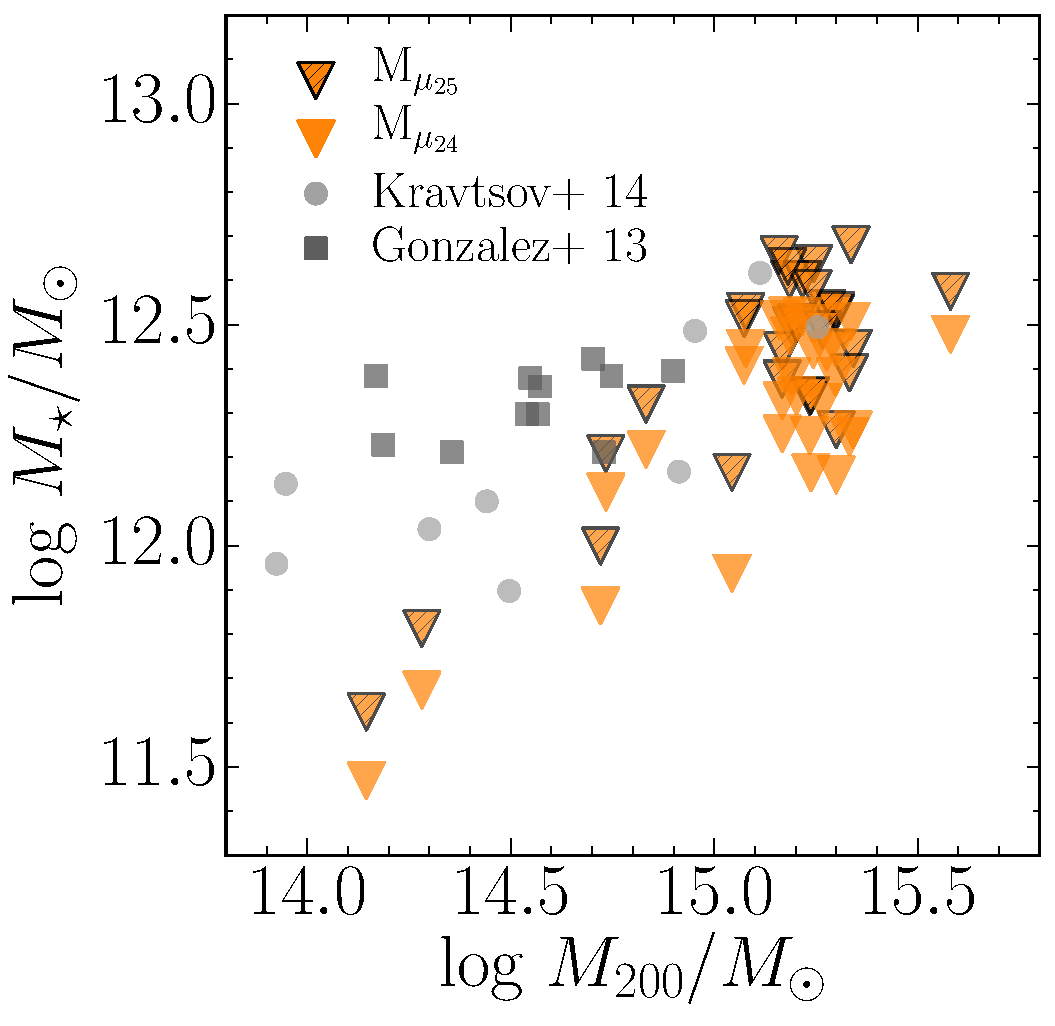
\includegraphics[height=12cm,width=12cm]{Figures/LR/Mbcg_vs_M200.pdf}
%\decoRule
\caption[mbcg]{}
\label{fig:mbcg}
\end{figure}

\begin{figure}[H]
\centering
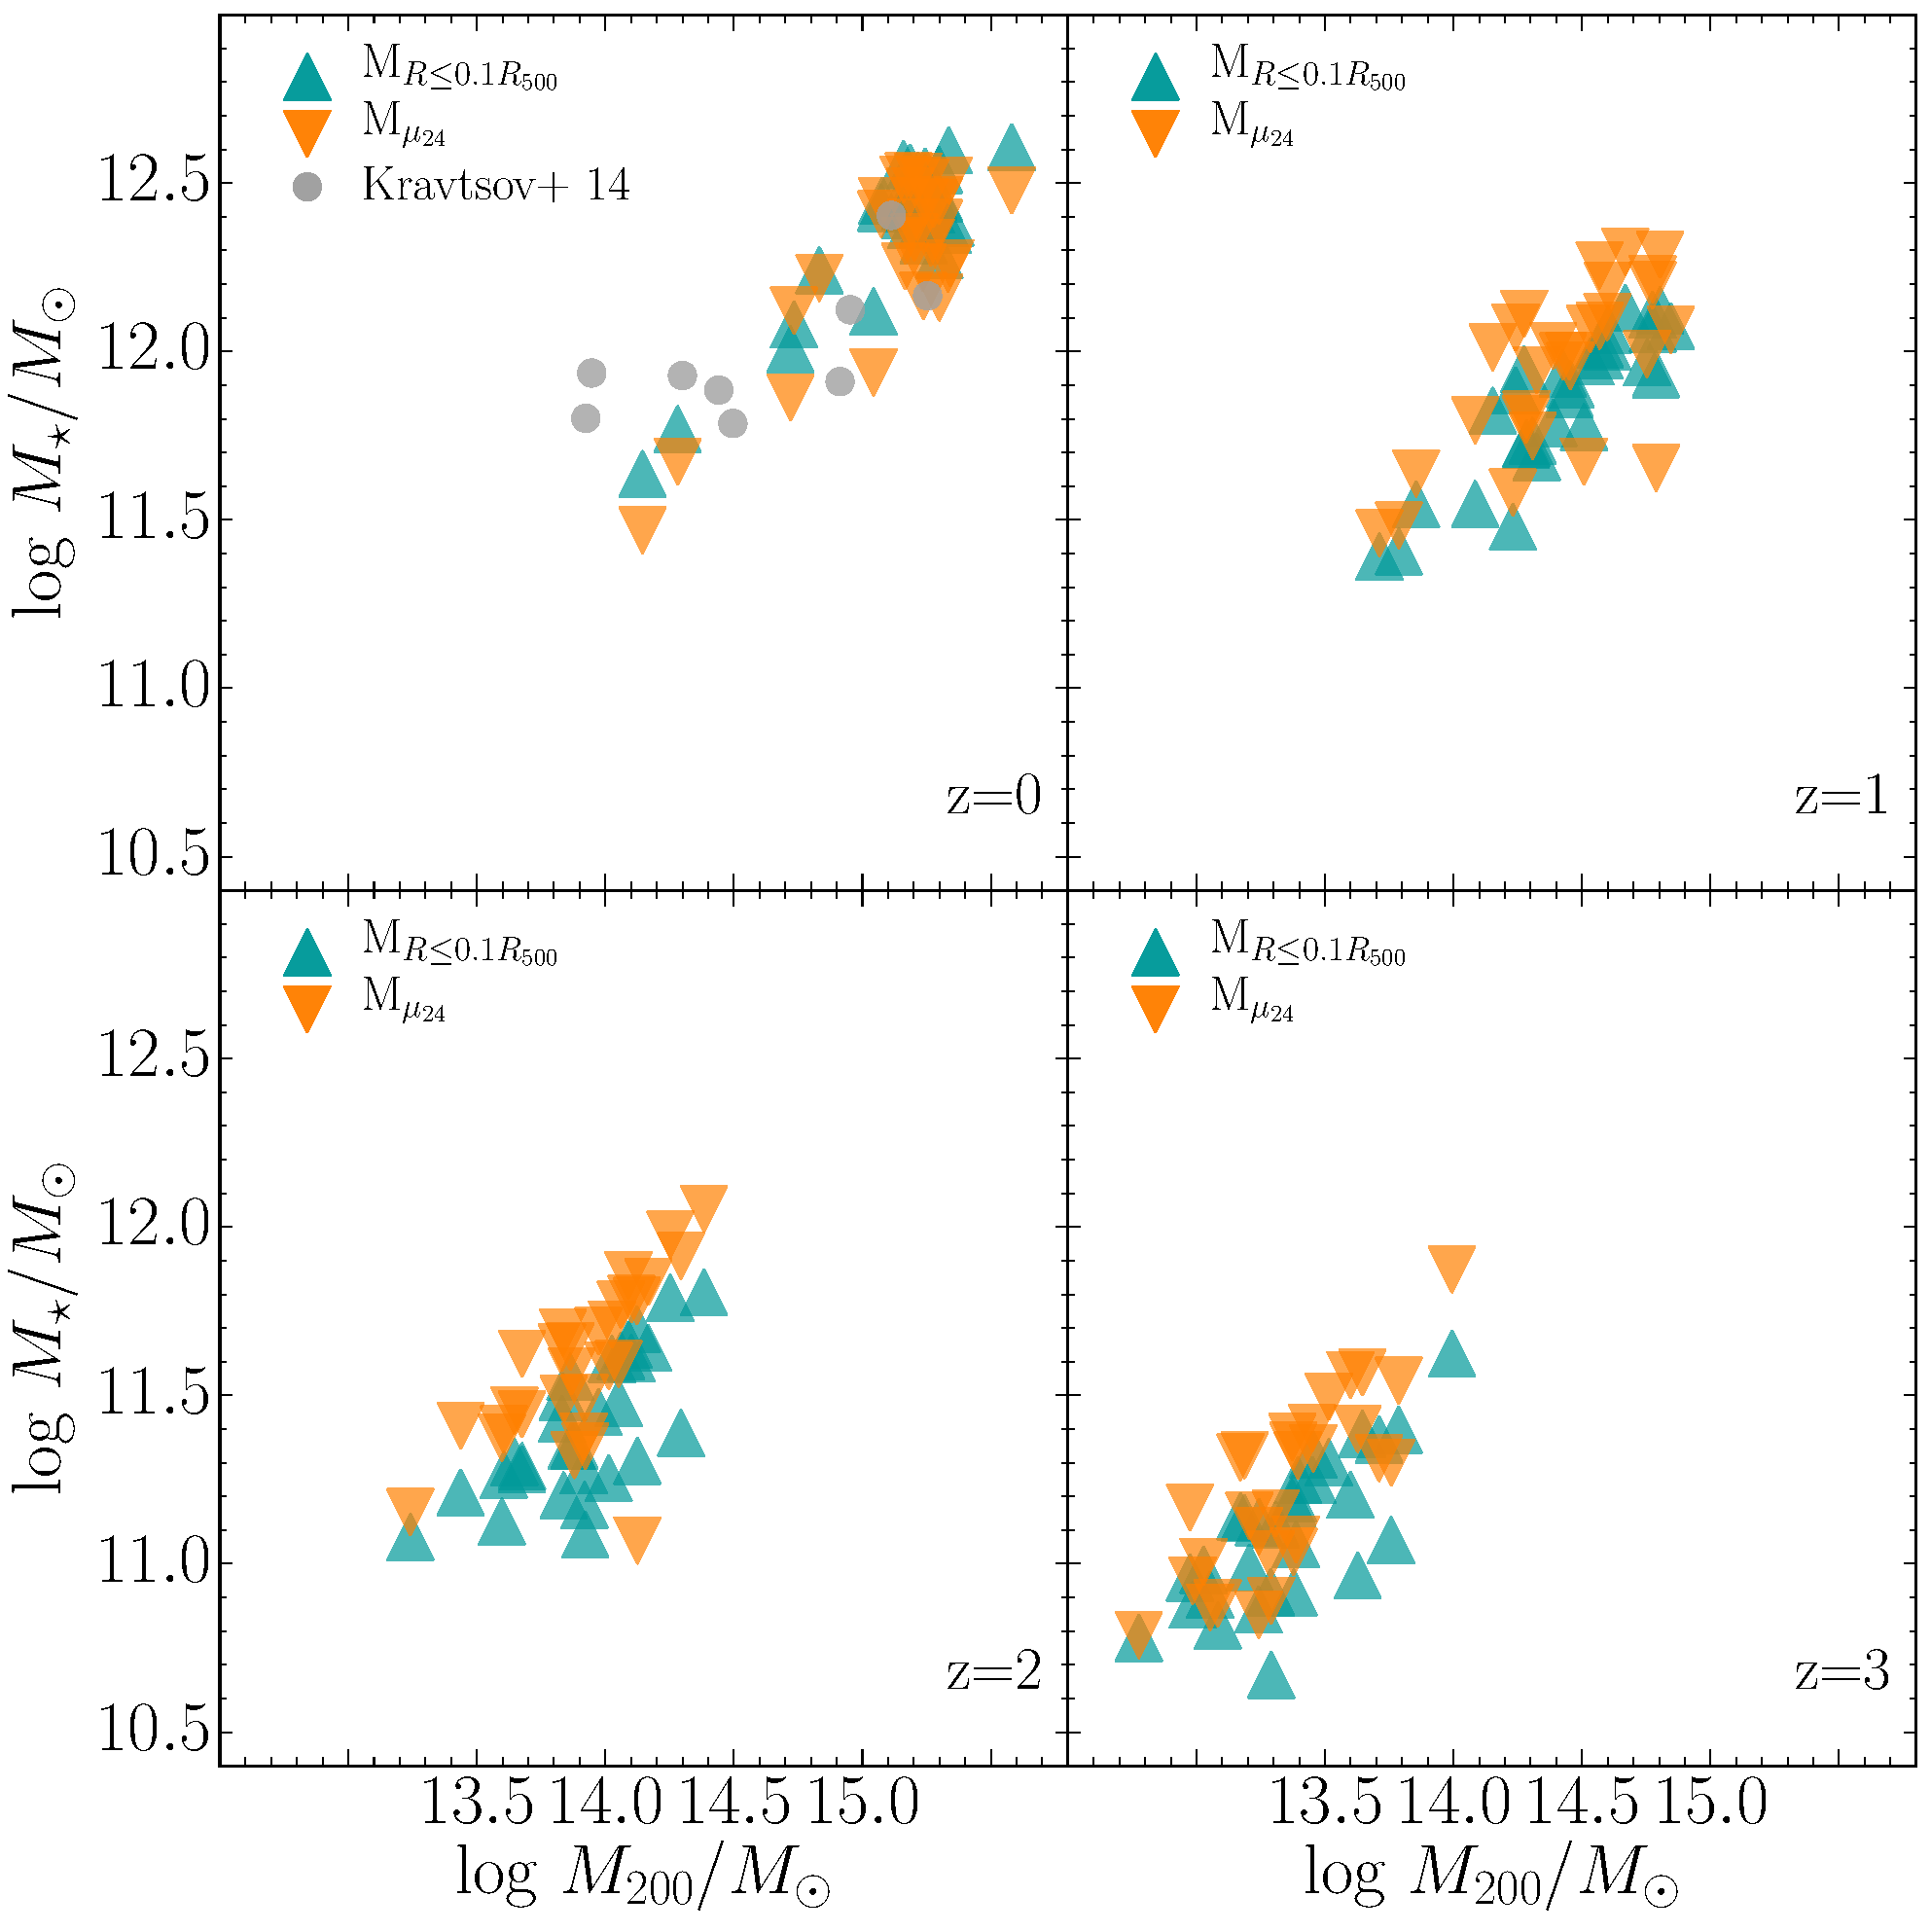
\includegraphics[height=12cm,width=12cm]{Figures/LR/muvs10r.pdf}
%\decoRule
\caption[muvs10r500]{}
\label{fig:muvs10r500}
\end{figure}

\begin{figure}[H]
\centering
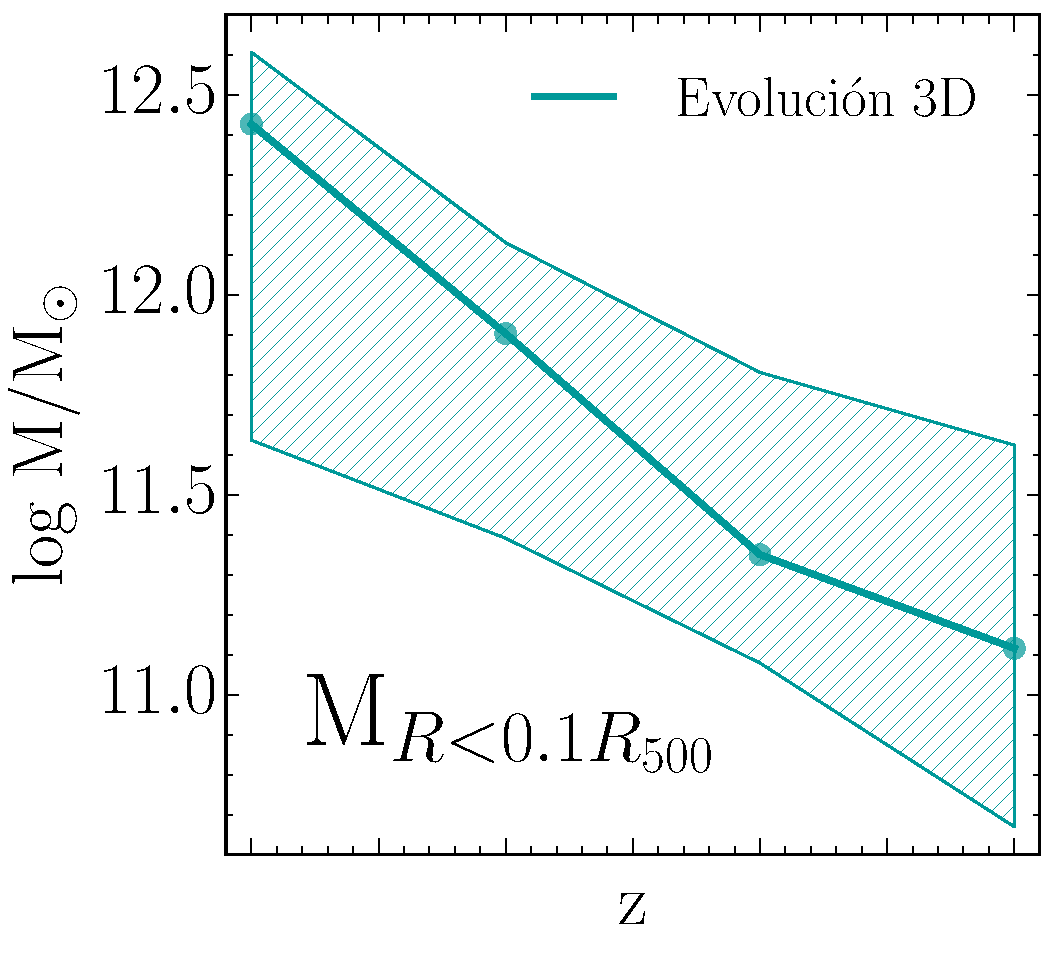
\includegraphics[height=12cm,width=12cm]{Figures/LR/evolucion_m10.pdf}
%\decoRule
\caption[evom10]{}
\label{fig:evom10}
\end{figure}

\begin{figure}[H]
\centering
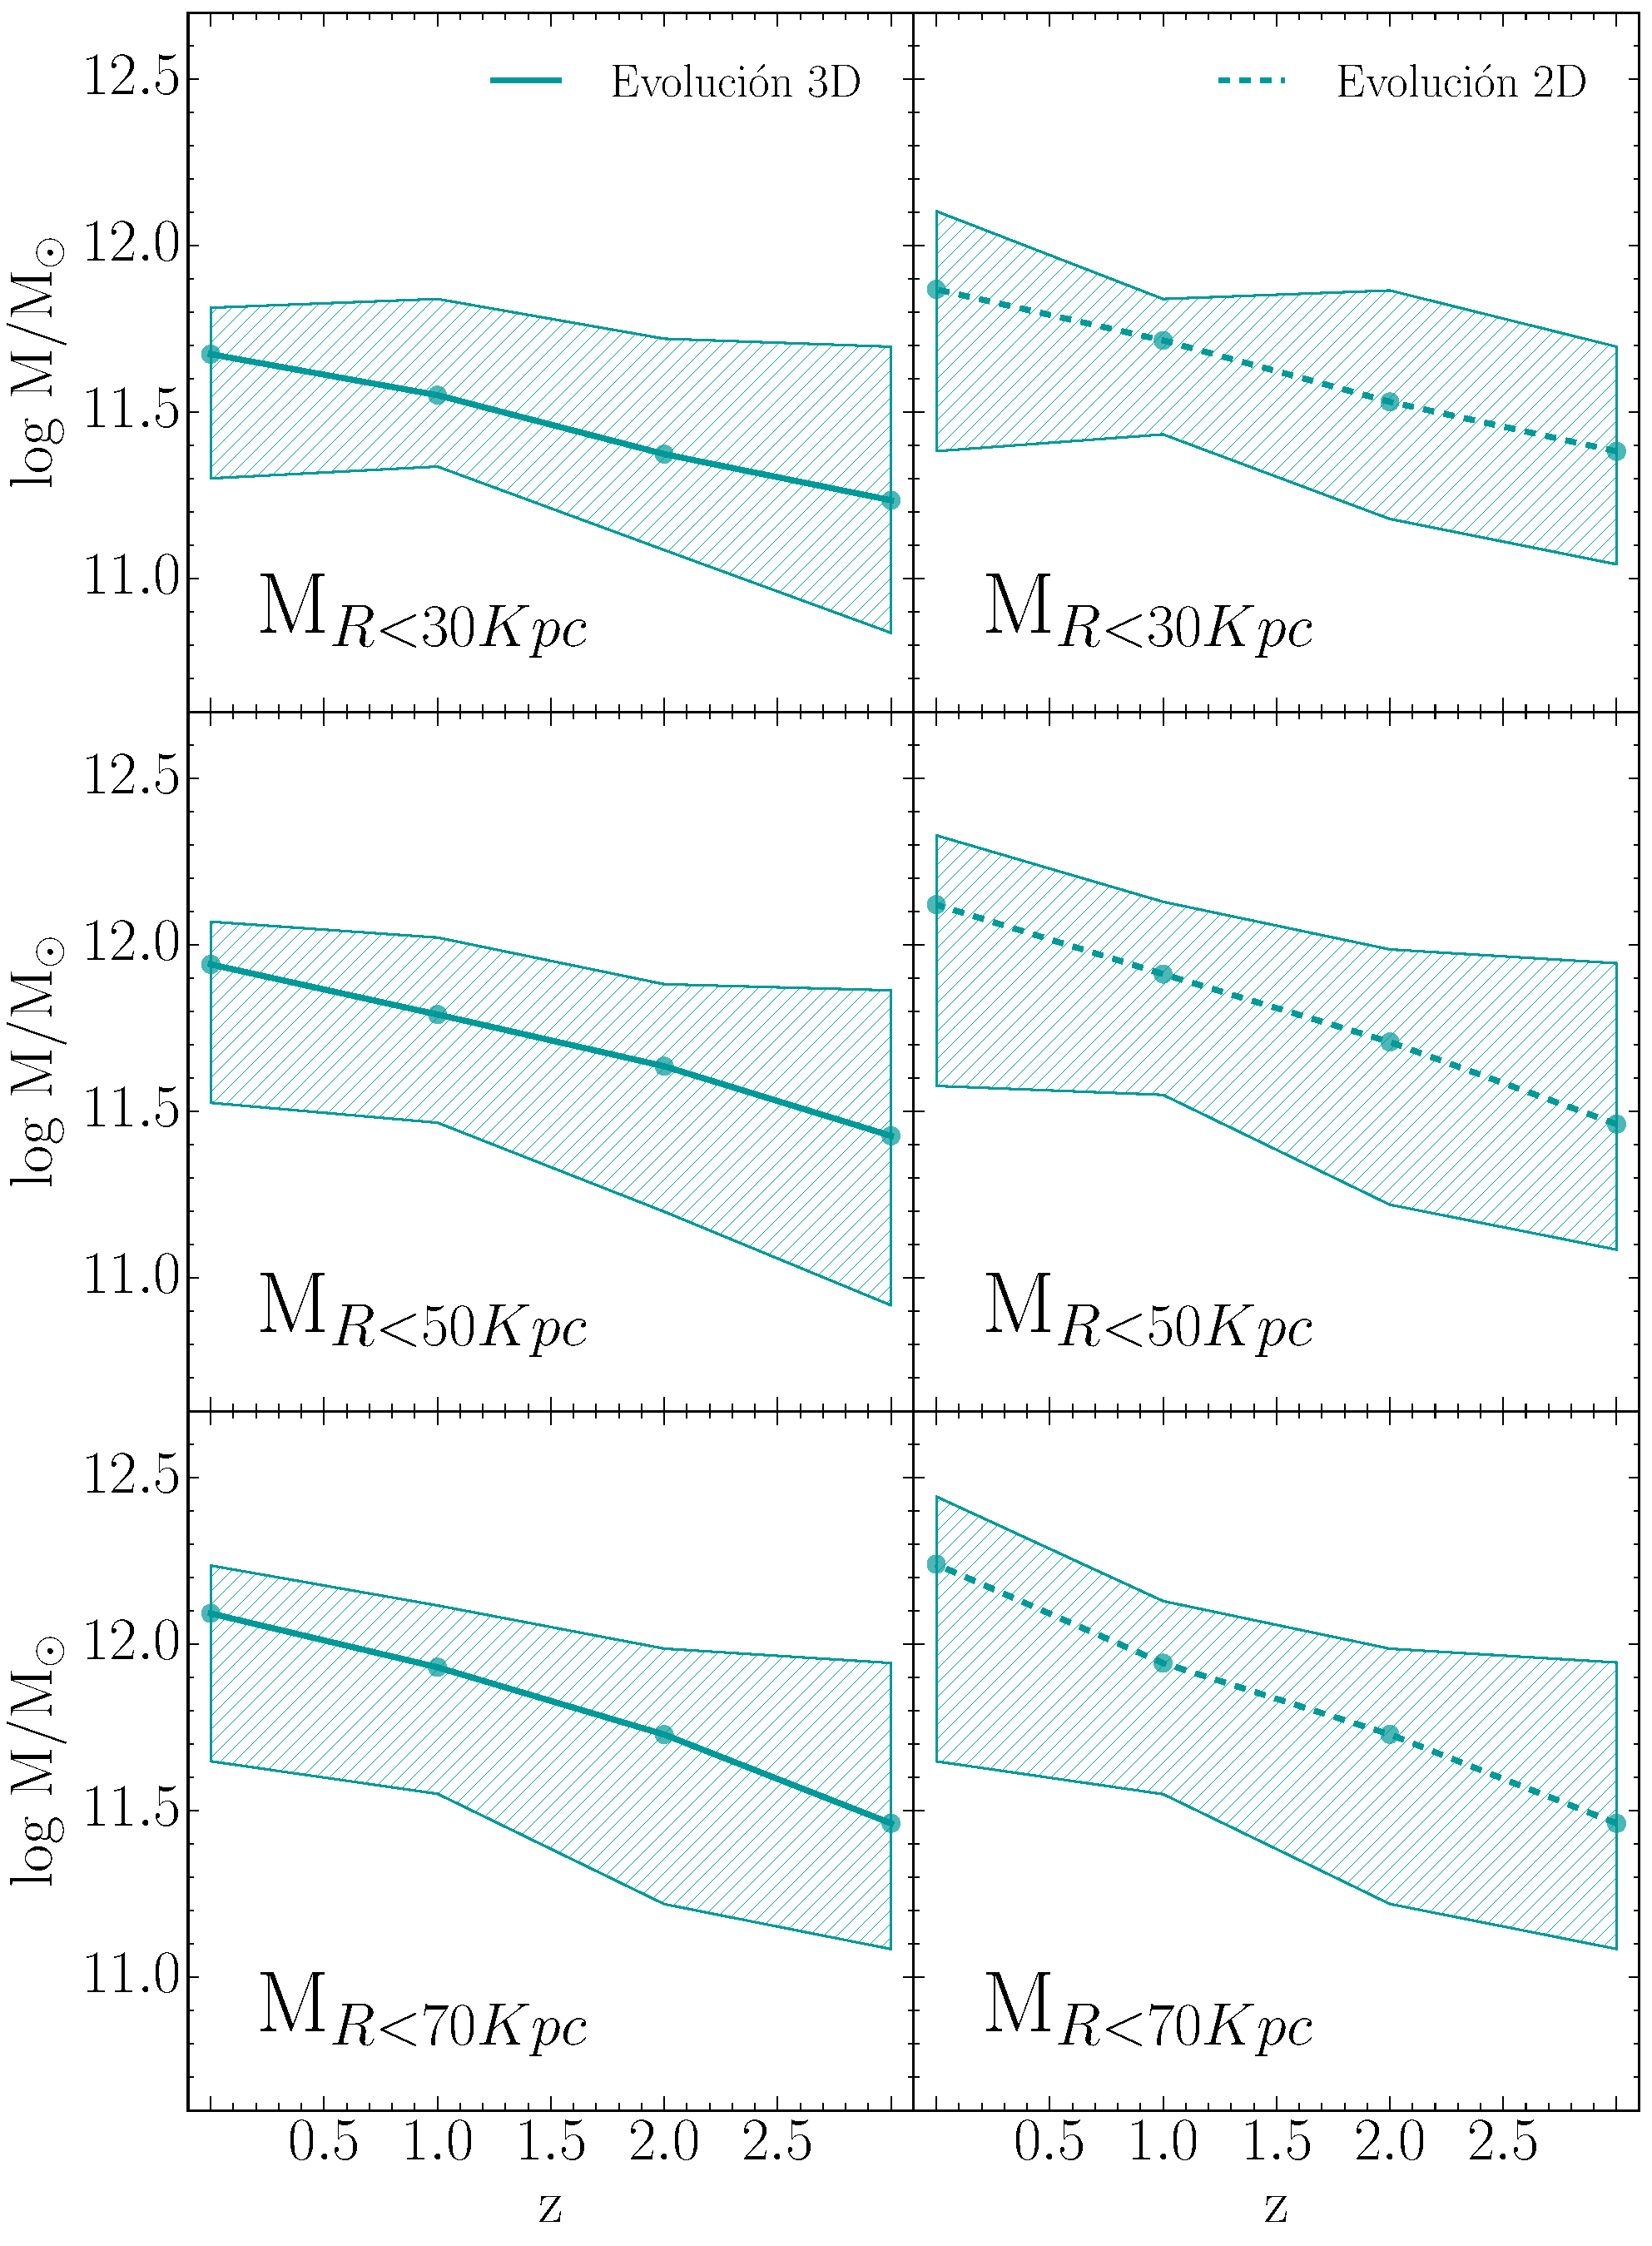
\includegraphics[height=17cm,width=12cm]{Figures/LR/evolucion.pdf}
%\decoRule
\caption[evol]{}
\label{fig:evol}
\end{figure}


\begin{figure}[H]
\centering
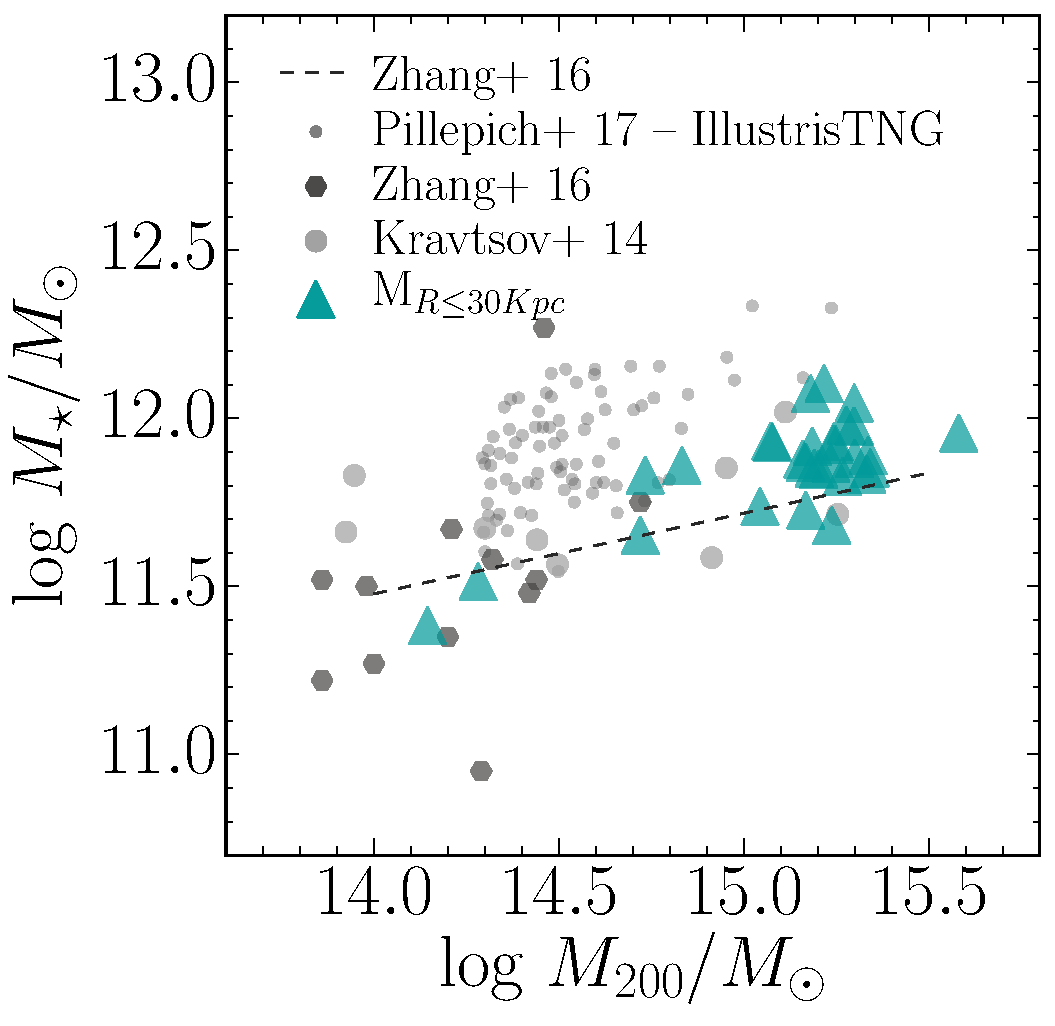
\includegraphics[height=12cm,width=12cm]{Figures/LR/M302D_vs_M200.pdf}
%\decoRule
\caption[mbcg]{}
\label{fig:m30}
\end{figure}


\begin{figure}[H]
\centering
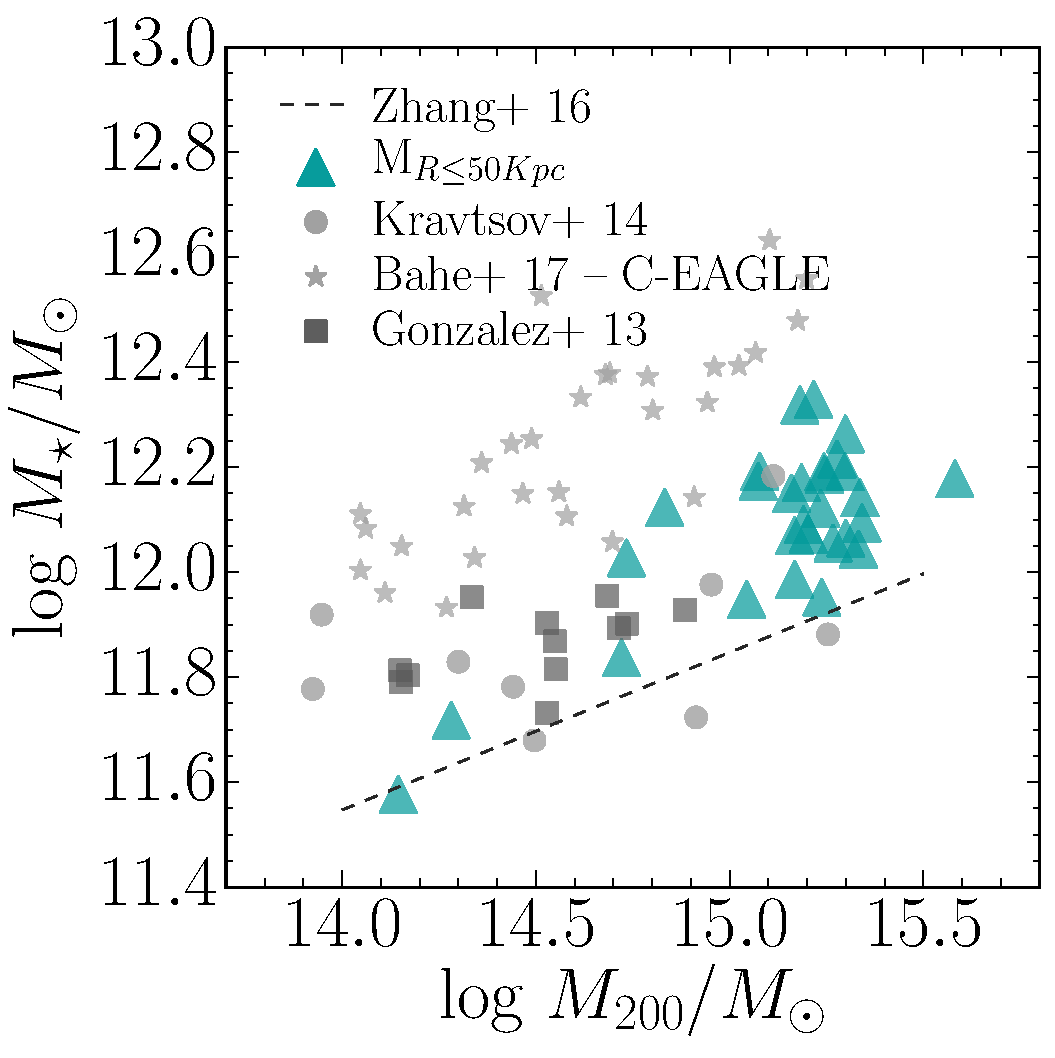
\includegraphics[height=12cm,width=12cm]{Figures/LR/M502D_vs_M200.pdf}
%\decoRule
\caption[mbcg]{}
\label{fig:m50}
\end{figure}


\begin{figure}[H]
\centering
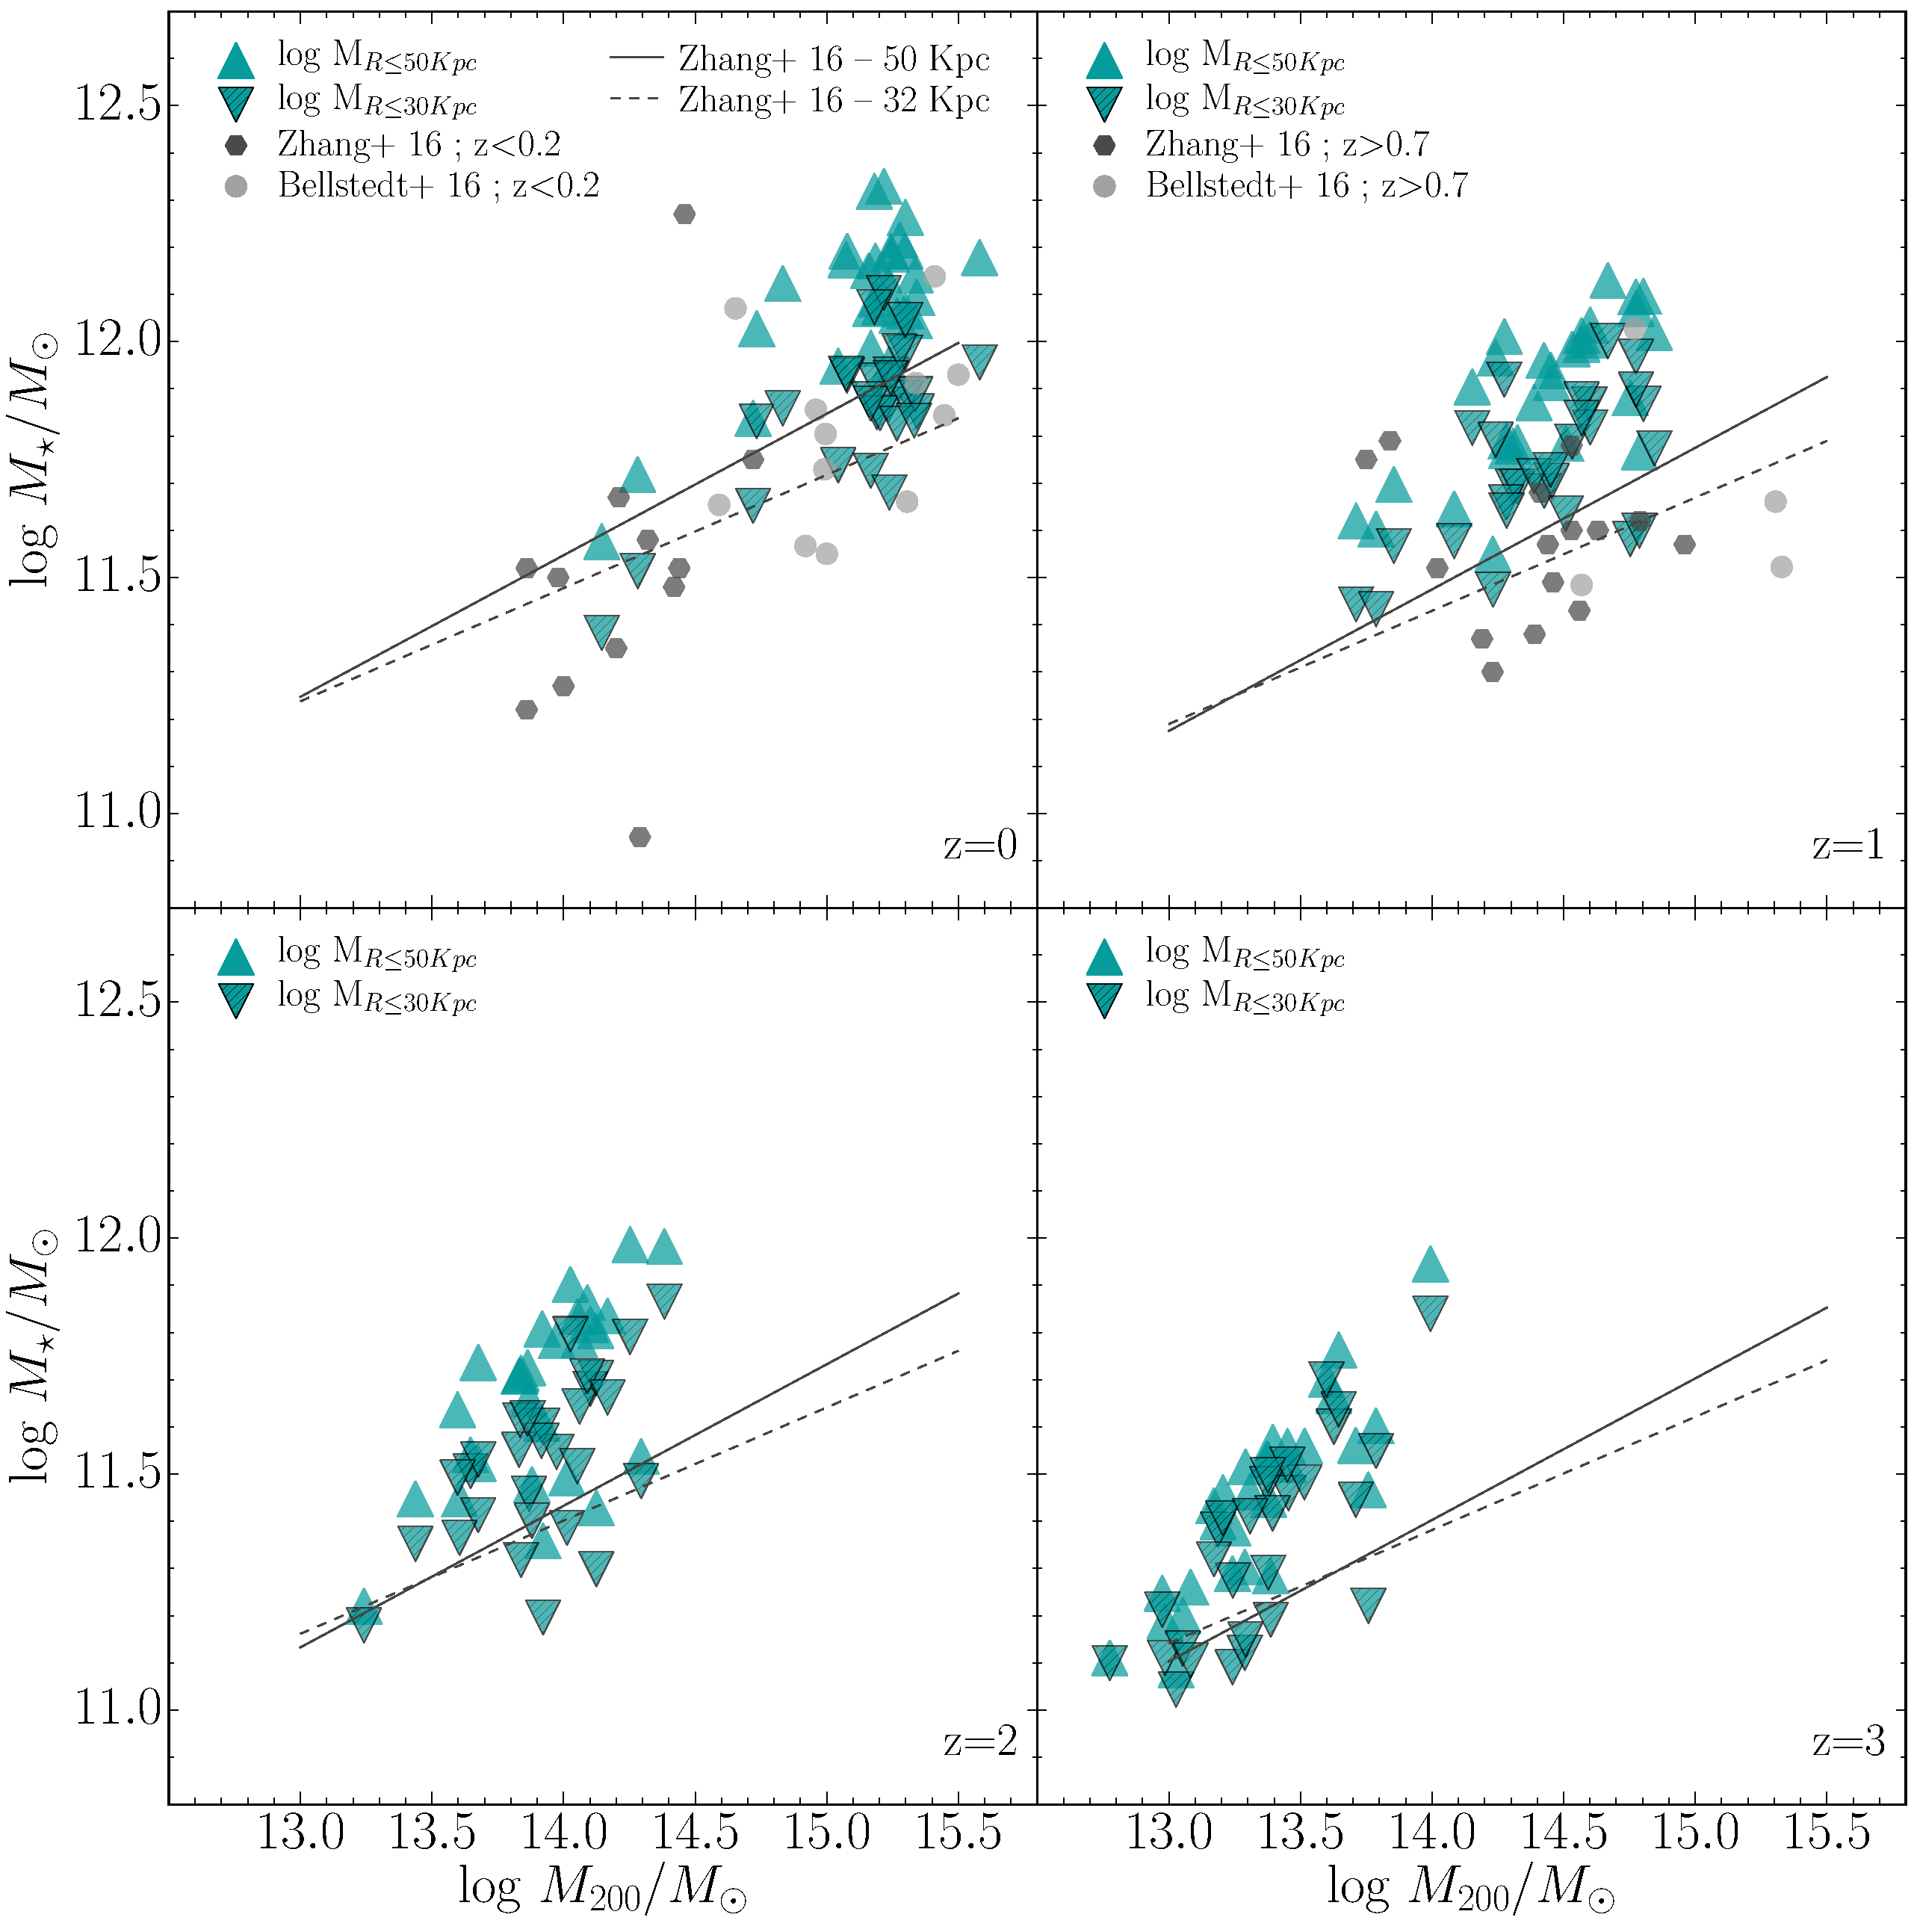
\includegraphics[height=12cm,width=12cm]{Figures/LR/zhang_vs_z.pdf}
%\decoRule
\caption[zhang]{}
\label{fig:zhang}
\end{figure}

%----------------------------------------------------------------------------------------
\section{Evoluci\'on Taman\~no}
%----------------------------------------------------------------------------------------
\section{Influencia del Polvo}
%----------------------------------------------------------------------------------------
\section{Estabilidad a Mayor Resoluci\'on}
%----------------------------------------------------------------------------------------